\documentclass{beamer}

%\usetheme[frameno]{Arguelles}
%\usetheme{default}
\usetheme{Madrid}
\usetheme{default}
\usepackage{svg}
%\usepackage{minted}
\usepackage{adjustbox}
\usepackage{listings}
\usepackage{hyperref}

% \usepackage[utf8]{inputenc}
% \usepackage[russian]{babel}
\usepackage{graphicx}
\usepackage{blkarray}
% \usepackage{sidecap}
\usepackage{csquotes}
\usepackage{amsmath}
\usepackage{emoji}
\usepackage[backend=biber,hyperref=true,style=numeric]{biblatex}

% Установка цветов ссылок
\hypersetup{
    colorlinks=true,      % Включает цветные ссылки
    linkcolor=blue,      % Цвет ссылок на внутренние ссылки
    citecolor=blue,      % Цвет ссылок на цитаты
    urlcolor=blue        % Цвет ссылок на URL
}

% Настройки для Python кода
% Define style for Bash code
\lstdefinestyle{bashStyle}{
  language=Bash,
  basicstyle=\ttfamily\footnotesize,
  keywordstyle=\color{blue},
  commentstyle=\color{gray},
  stringstyle=\color{orange},
  showstringspaces=false,
  columns=flexible,
  numbers=left,
  numberstyle=\tiny\color{gray},
  backgroundcolor=\color{lightgray!20},
  frame=single,
  breaklines=true,
  captionpos=b,
  xleftmargin=1em,
  xrightmargin=1em
}

\hypersetup{
    colorlinks=true,
    linkcolor=blue,
    urlcolor=blue
}

% Define style for Python code
\lstdefinestyle{pythonStyle}{
  language=Python,
  basicstyle=\ttfamily\footnotesize,
  keywordstyle=\color{blue},
  commentstyle=\color{gray},
  stringstyle=\color{orange},
  showstringspaces=false,
  columns=flexible,
  numbers=left,
  numberstyle=\tiny\color{gray},
  backgroundcolor=\color{lightgray!20},
  frame=single,
  breaklines=true,
  captionpos=b,
  xleftmargin=1em,
  xrightmargin=1em
}

% Добавление поддержки русского языка
\usepackage[utf8]{inputenc} % UTF-8 кодировка
\usepackage[russian, english]{babel} % Поддержка русского и английского языков
\usepackage{tikz}

\title{NLP intro}
\subtitle{Overview}
\author{Vasily Konovalov, Andrei Glinskii}
\date{}
\addbibresource{./references.bib}


\begin{document}

\frame[plain]{\titlepage}

\section{Program}

\begin{frame}{Prerequisites}{}
    \begin{itemize}
        \item Python
        \item PyTorch
        \item Linear Algebra
        \item Multivariate Calculus
        \item Probability and Statistics
        \item Fundamentals of Machine Learning
    \end{itemize}
\end{frame}

\begin{frame}{Lectures}
    \begin{columns}
        \begin{column}{0.5\textwidth}
            \begin{itemize}
                \item 01 Intro
                \item 02 NLP basics
                \item 03 NN basics
                \item 04 Basic NN in NLP
                \item 05 RNN
                \item 06 Seq2seq, attention
            \end{itemize}
        \end{column}
        \begin{column}{0.5\textwidth}
            \begin{itemize}
                \item 07 Encoders
                \item 08 Decoders
                \item 09 LLM 1
                \item 10 LLM 2
                \item 11 Multimodality
                \item 12 Final test
            \end{itemize}
        \end{column}
    \end{columns}
\end{frame}

\begin{frame}{Sources}{}
    \begin{columns}
        \begin{column}{0.5\textwidth}
            \begin{itemize}
                \item \href{https://www.amazon.com/Natural-Language-Processing-Transformers-Applications/dp/1098103246}{NLP with Transformers}
                \item \href{https://probml.github.io/pml-book/}{Probabilistic Machine Learning Book}
                \item \href{https://udlbook.github.io/udlbook/}{Understanding Deep Learning Book}
                \item \href{https://www.deeplearningbook.org/}{Deep Learning Book}
                \item \href{https://nn.labml.ai/}{LabML.ai}
                \item \href{https://huggingface.co/blog}{Hugging Face Blog}
            \end{itemize}
        \end{column}
        \begin{column}{0.5\textwidth}
            \begin{itemize}
                \item \href{https://www.youtube.com/@AndrejKarpathy}{Andrej Karpathy}
                \item \href{https://www.youtube.com/@umarjamilai}{Umar Jamil}
                \item \href{https://www.youtube.com/@statquest}{StatQuest}
                \item \href{https://www.youtube.com/@3blue1brown}{3Blue1Brown}
                \item \href{https://lena-voita.github.io/}{Lena Voita}
                \item \href{https://lilianweng.github.io/}{Lilian Weng}
                \item \href{https://neurips.cc/}{NeurIPS}, \href{http://cvpr2024.thecvf.com/}{CVPR}, \href{https://icml.cc/}{ICML}, \href{http://iccv2023.thecvf.com/}{ICCV/ECCV}, \href{https://iclr.cc/}{ICLR}, \href{https://www.aclweb.org/portal/}{ACL}, \href{https://aaai.org/}{AAAI}, \href{https://2024.emnlp.org/}{EMNLP}
            \end{itemize}
        \end{column}
    \end{columns}
\end{frame}


\begin{frame}{NLP research topics}
\begin{itemize}
        \item Hallusinations
        \begin{itemize}
        \item Evaluation
        \item Mitigation
        \item incl LVLM and Code-based LLM
        \item incl based on Knowledge Bases
        \end{itemize}
        \item Uncertainty Estimation (belikova)
        \item Representation Editing
        \item LM context increasing methods (bulatov2023scaling)
        \item LM interpretation methods
    \end{itemize}
\end{frame}

\begin{frame}{Grading Policy}{}
    \begin{itemize}
        \item Home works
        \item Tests
        \item Final test
        \item Attendance
    \end{itemize}
\end{frame}

\section{Introduction to NLP}

\begin{frame}{NLP as interdisciplinary field}{}
    \begin{figure}
        \centering
        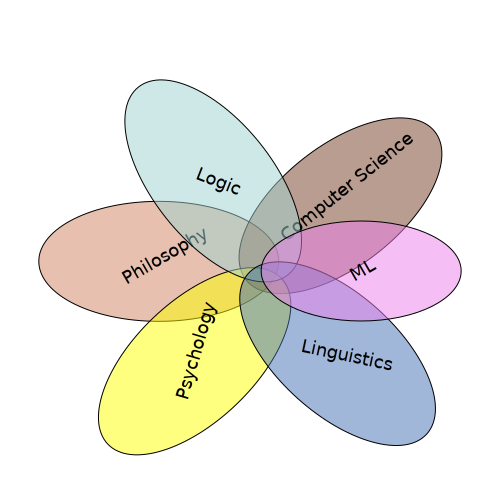
\includegraphics[width=0.7\textwidth,keepaspectratio]{images/interdisciplinary_field}
%        \caption{}
        \label{fig:interdisciplinary_field}
    \end{figure}
\end{frame}

\begin{frame}{NLP as a part of AI}{}
    \begin{figure}
        \centering
        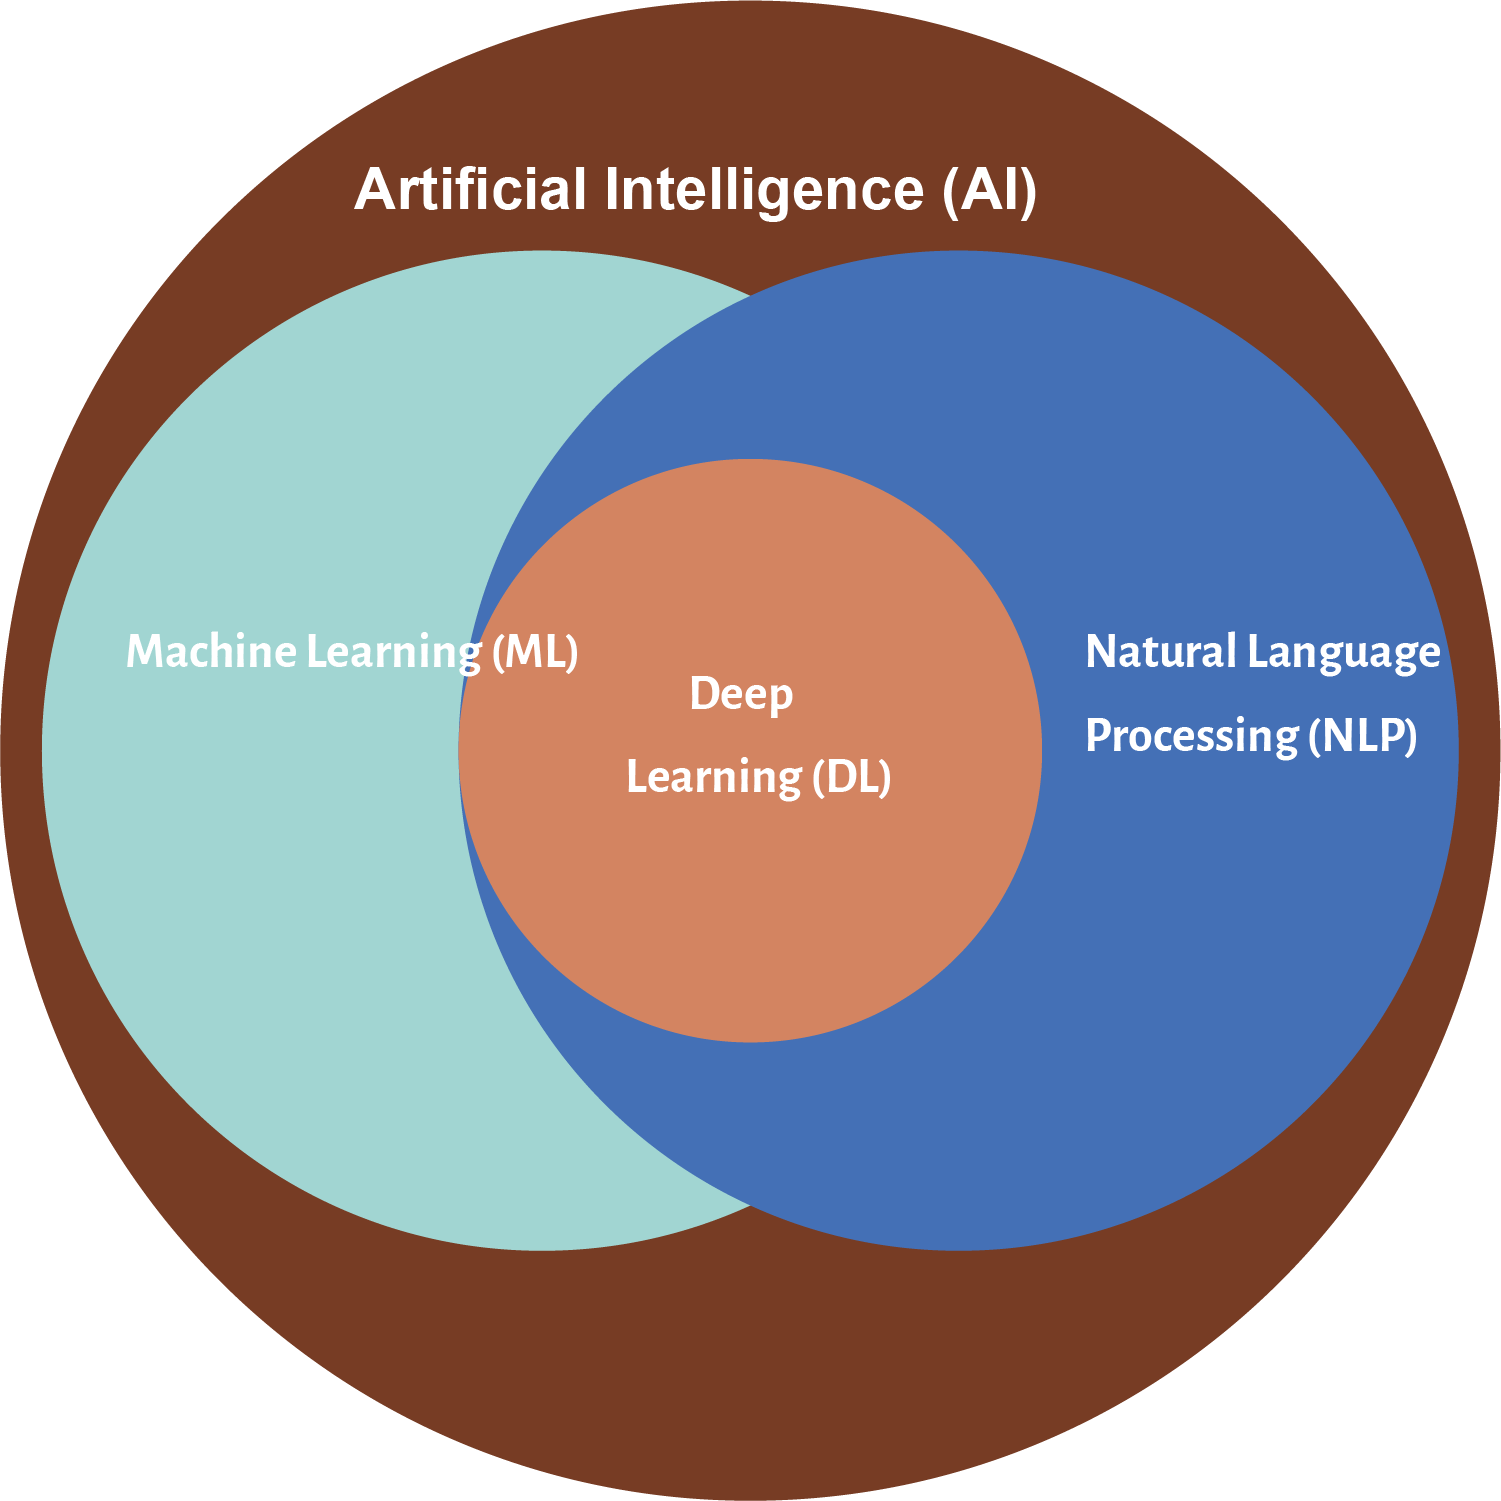
\includegraphics[width=0.7\textwidth,keepaspectratio]{images/nlp_diagram}
%        \caption{}
        \label{fig:nlp_diagram}
    \end{figure}
\end{frame}

\begin{frame}{Introduction}
    \begin{columns}
        \begin{column}{0.5\textwidth}
            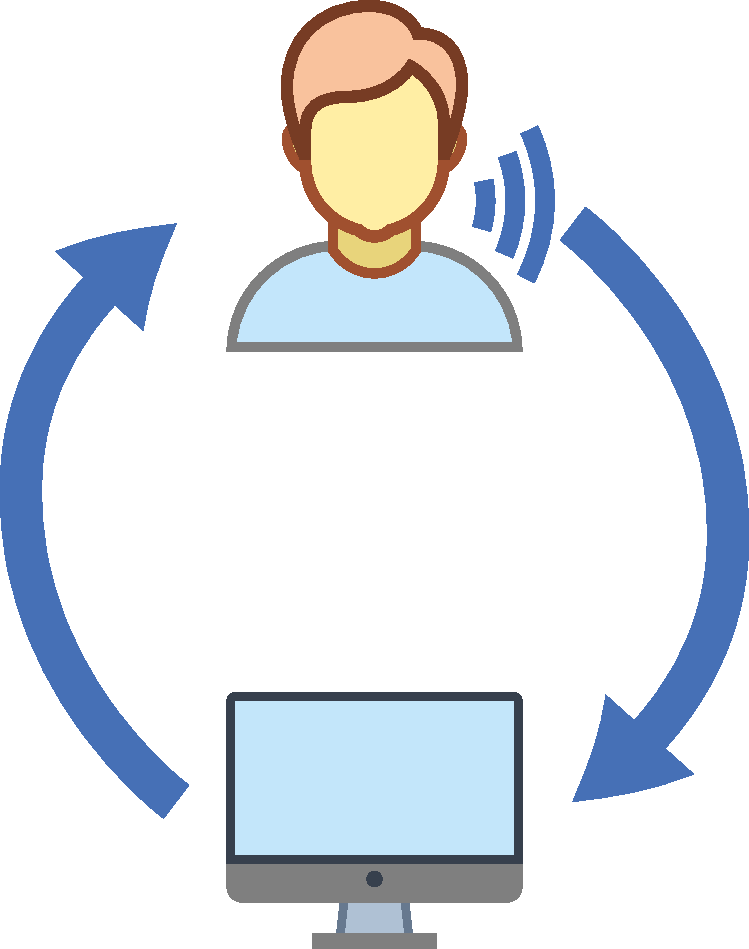
\includegraphics[width=\linewidth,keepaspectratio]{images/human_computer_interaction}
%            \caption{}
            \label{fig:human_computer_interaction}
        \end{column}
        \begin{column}{0.5\textwidth}
            \begin{itemize}
                \item Chatbots and Virtual Assistants
                \item Machine Translation
                \item Information Extraction
                \item Speech Recognition
                \item Text Summarization
                \item Sentiment Analysis
                \item Morphology
                \item \text{...}
            \end{itemize}
        \end{column}
    \end{columns}
\end{frame}

\begin{frame}
\frametitle{Simple task example - morphological analysis}
\begin{itemize}
    \item Morphological analysis, stemming, and lemmatization are essential techniques in Natural Language Processing (NLP).
    \item They are used to process and understand text by breaking down words and identifying their base forms.
    \item These techniques help in text normalization, which is crucial for tasks such as search and information retrieval.
\end{itemize}
\end{frame}

\begin{frame}
\frametitle{Morphological Analysis}
\begin{itemize}
    \item Morphological analysis involves examining the structure of words to understand their meaning and relationships.
    \item It breaks words into their constituent morphemes (the smallest meaningful units).
    \item Example: The word "unhappily" can be broken down into "un-", "happy", and "-ly".
\end{itemize}
\end{frame}

\begin{frame}
\frametitle{Stemming}
\begin{itemize}
    \item Stemming is the process of reducing a word to its root or base form.
    \item It removes suffixes and prefixes to obtain a common base form.
    \item Example: "running", "runner", and "ran" are all reduced to "run".
    \item Algorithms: Porter Stemmer, Snowball Stemmer.
\end{itemize}
\end{frame}

\begin{frame}
\frametitle{Lemmatization}
\begin{itemize}
    \item Lemmatization is the process of reducing a word to its base or dictionary form (lemma).
    \item Unlike stemming, lemmatization considers the context and part of speech.
    \item Example: "better" is lemmatized to "good".
    \item Requires a lexicon and part-of-speech tagging.
\end{itemize}
\end{frame}

\begin{frame}
\frametitle{Comparison: Stemming vs. Lemmatization}
\begin{itemize}
    \item Stemming:
        \begin{itemize}
            \item Faster and less complex.
            \item May produce non-words.
        \end{itemize}
    \item Lemmatization:
        \begin{itemize}
            \item More accurate and context-aware.
            \item Requires more computational resources.
        \end{itemize}
\end{itemize}
\end{frame}

\begin{frame}
\frametitle{Complex task example - building LLM}
\begin{itemize}
  \item Language modeling
  \item Data collection and preprocessing
  \item Model architecture design
  \item Training and fine-tuning
  \item Evaluation metrics and validation
  \item Deployment options
  \item Fine-tuning for specific use cases
  \item Optimizing performance and efficiency
  \item Integrating language models with applications
  \item \text{...}
\end{itemize}
\end{frame}

\begin{frame}{LLMs}{}
    \begin{figure}
        \centering
        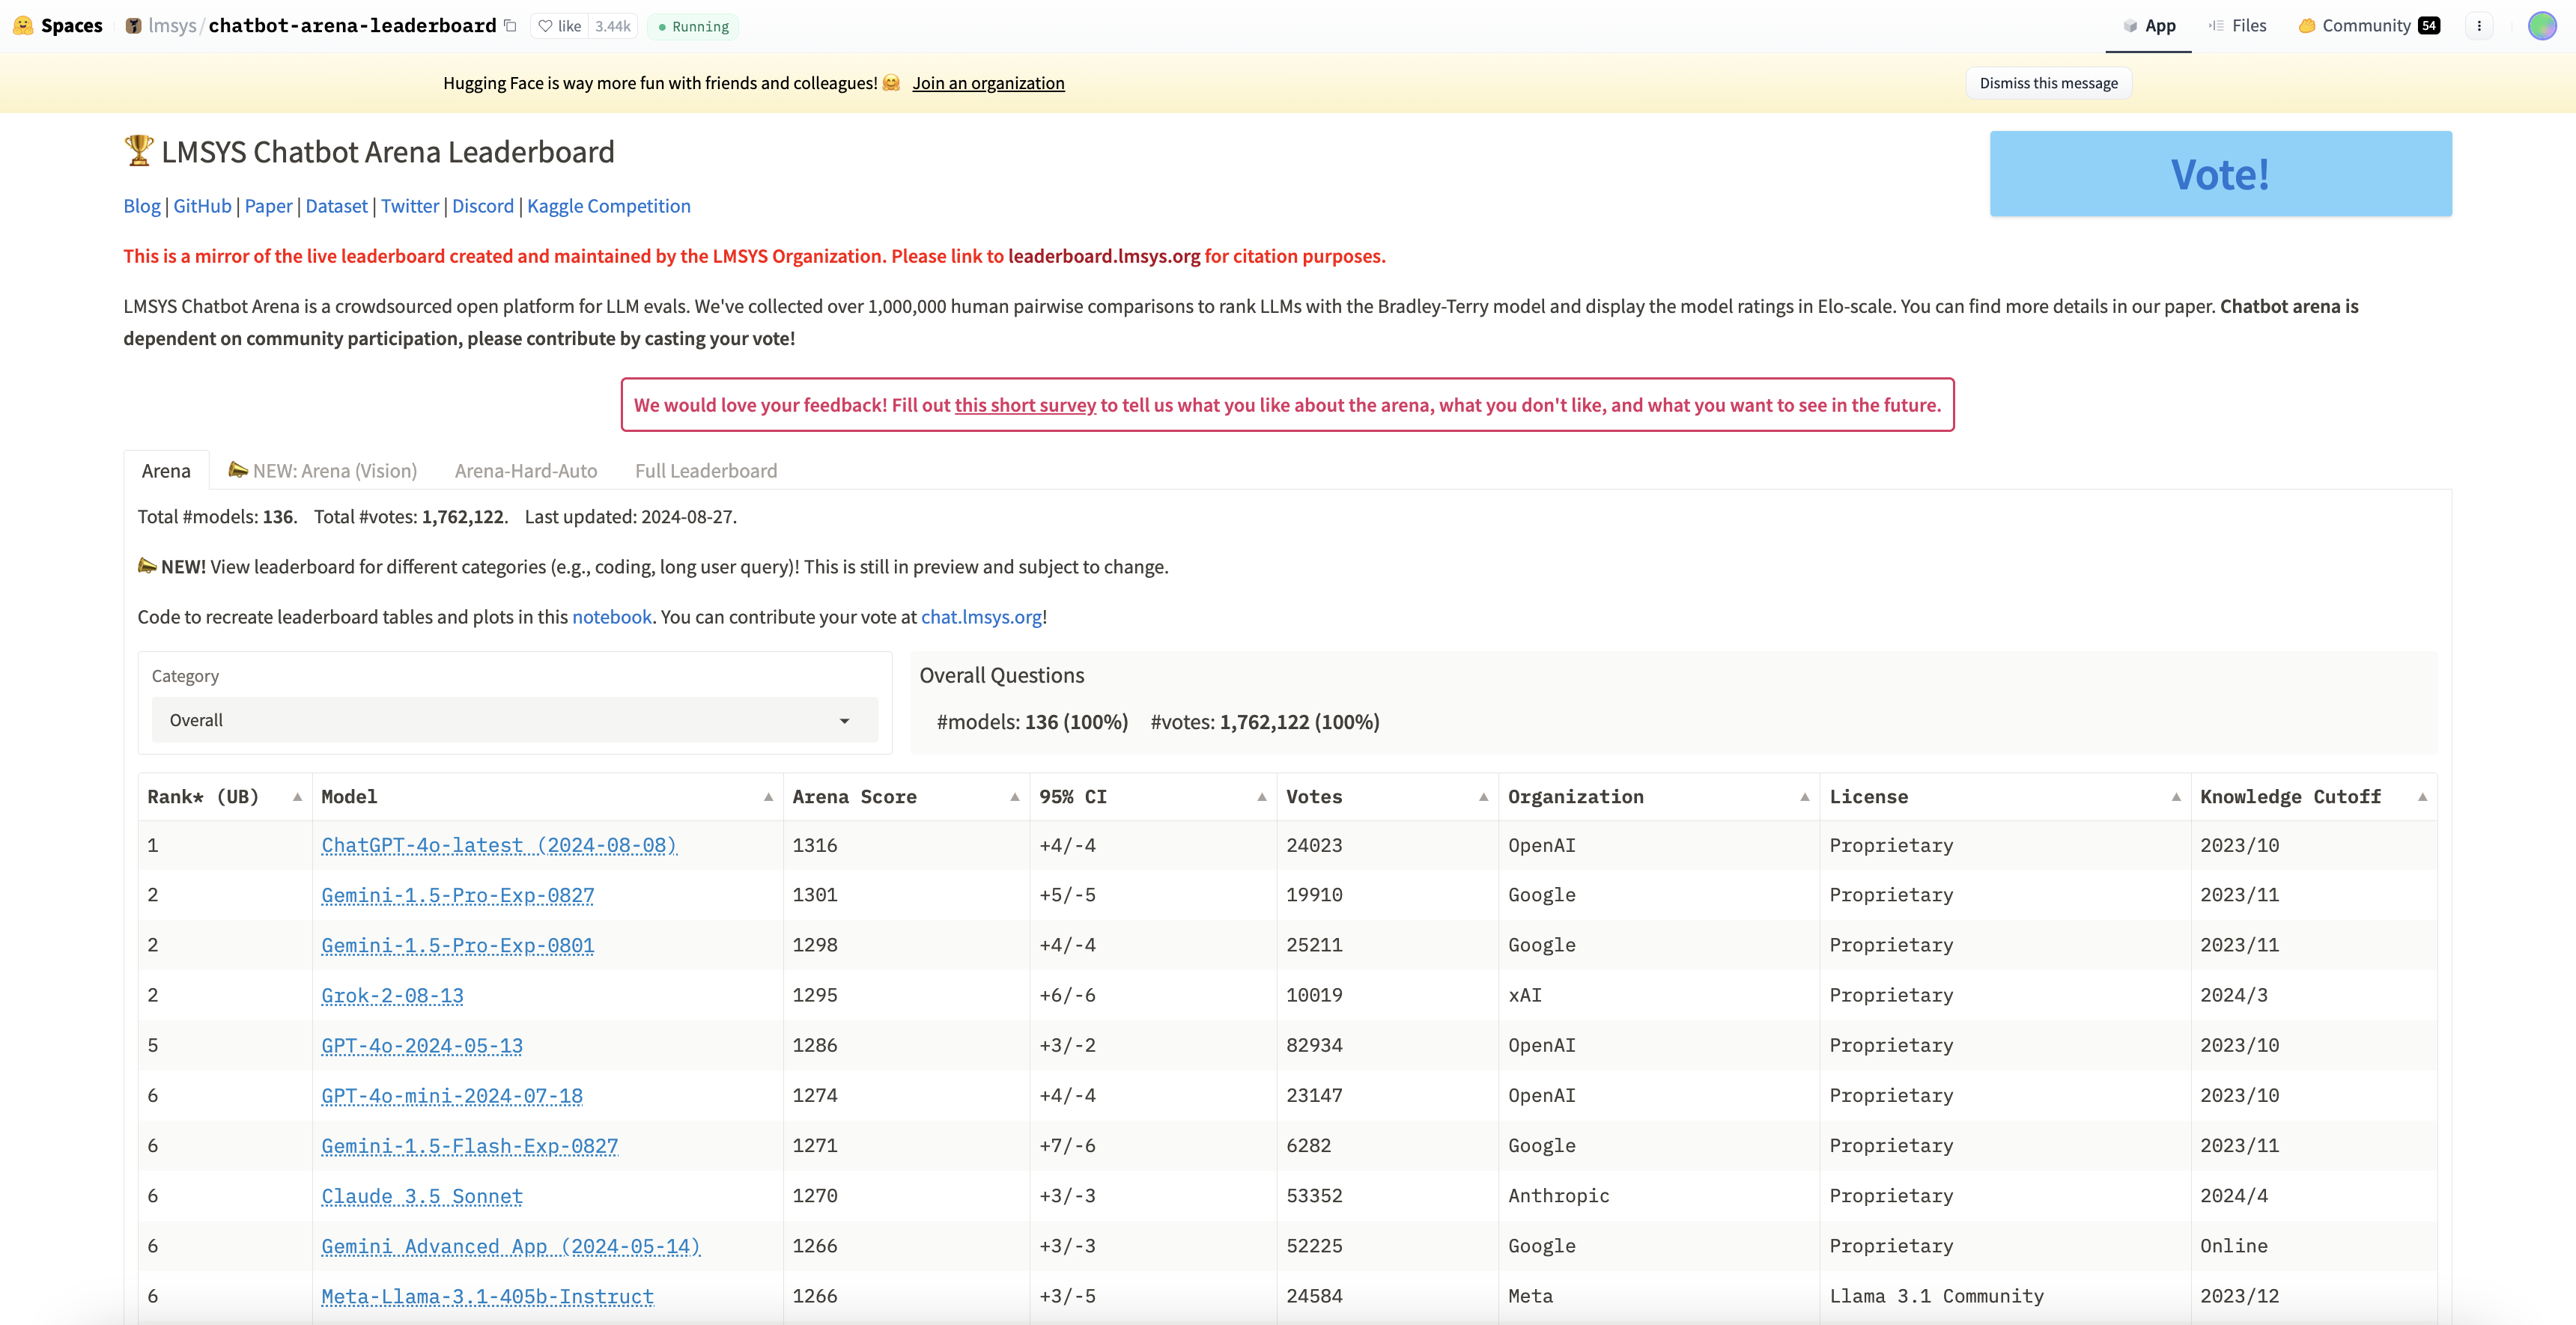
\includegraphics[width=1\textwidth,keepaspectratio]{images/chatbot_leaderboard}
%        \caption{}
        \label{fig:}
    \end{figure}
\end{frame}

\section{Basic NLP pipeline steps}

\begin{frame}
\frametitle{Building Language Models}
Natural Language Processing (NLP) is crucial for creating intelligent language models

Key concepts:
    \begin{itemize}
        \item Data collection
        \item Preprocessing
        \item Tokenization
        \item Language modeling
        \item Inference
    \end{itemize}
\end{frame}


\begin{frame}
\frametitle{Data Collection and Preprocessing}
\begin{itemize}
    \item Collect diverse dataset of text
    \item Preprocessing steps:
    \begin{itemize}
        \item Tokenization
        \item Stopwords removal
        \item Lemmatization
        \item Named Entity Recognition (NER)
        \item Sentiment analysis
        \item Data augmentation
    \end{itemize}
\end{itemize}
\end{frame}

\begin{frame}
\frametitle{Model Architecture Design}
\begin{itemize}
    \item Recurrent Neural Networks (RNNs)
    \item Transformer Models
    \item Hybrid Architectures
    \item Attention Mechanisms
\end{itemize}
\end{frame}

\begin{frame}
\frametitle{Choosing the Right Framework}
\begin{figure}
    \centering
    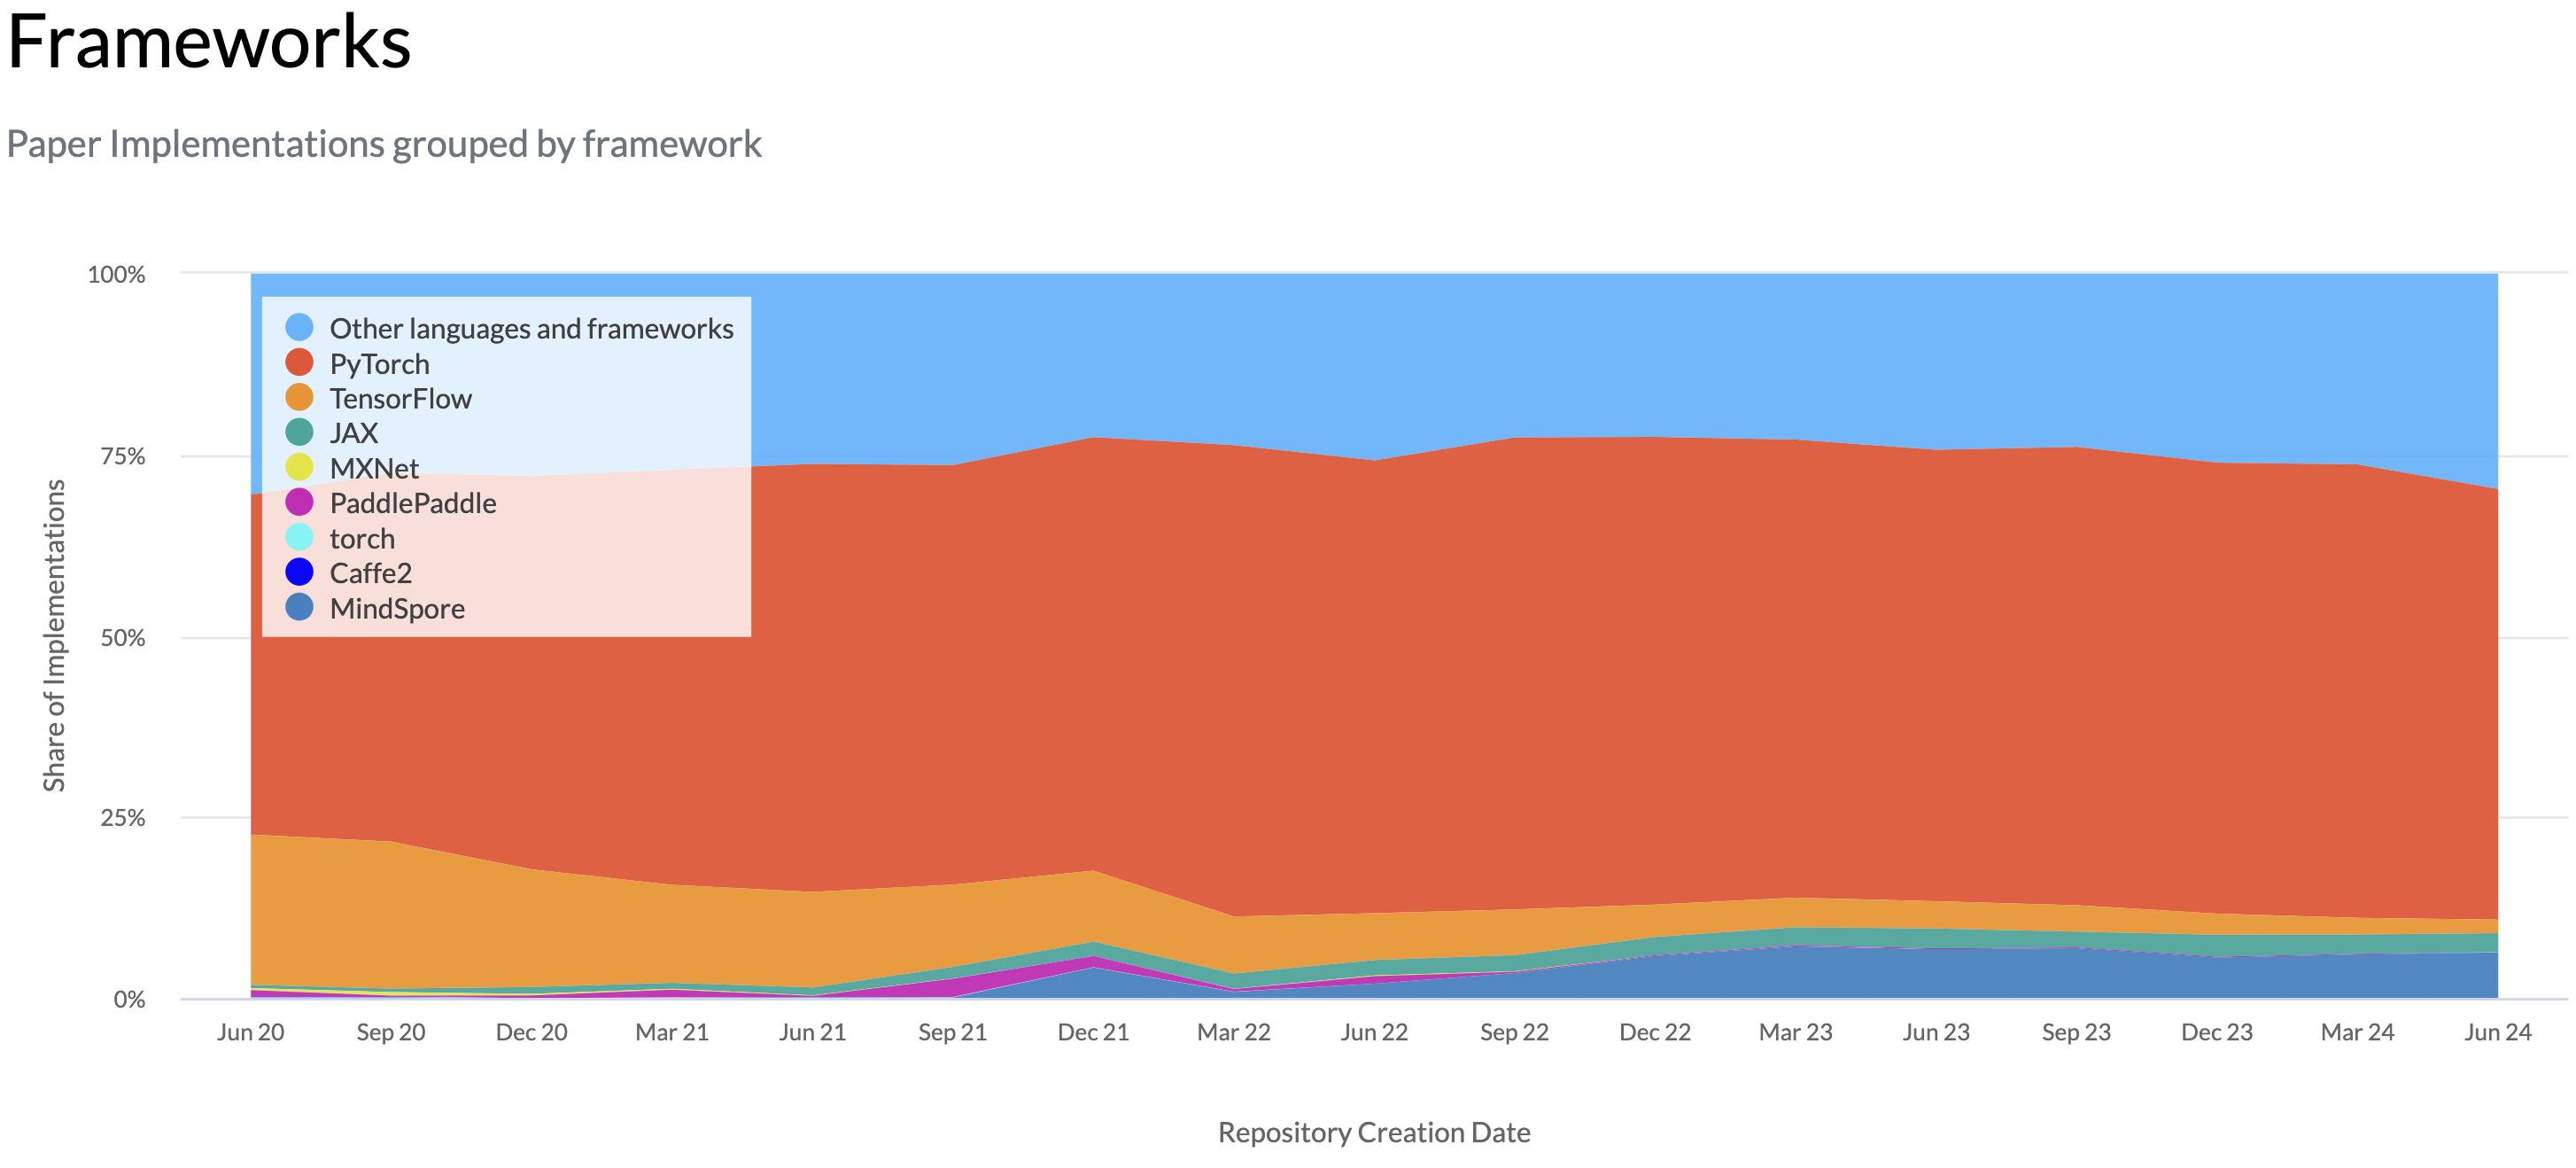
\includegraphics[width=1\textwidth,keepaspectratio]{images/frameworks}
    \caption{https://paperswithcode.com/trends}
    \label{fig:frameworks}
\end{figure}
\end{frame}

\begin{frame}
\frametitle{Framework Selection Criteria}
\begin{itemize}
    \item Project requirements
    \item Development experience
    \item Computational resources
    \item Model complexity
    \item Scalability
\end{itemize}
\end{frame}

\begin{frame}
\frametitle{Training and Fine-Tuning}
\begin{columns}
    \column{0.5\textwidth}
    \textbf{Techniques}
    \begin{itemize}
        \item Data augmentation
        \item Regularization
        \item Batch size optimization
        \item Learning rate scheduling
    \end{itemize}

    \column{0.5\textwidth}
    \textbf{Challenges}
    \begin{itemize}
        \item Overfitting
        \item Early stopping
        \item Weight regularization
        \item Transfer learning
    \end{itemize}
\end{columns}
\end{frame}

\begin{frame}
\frametitle{Metrics for Evaluating Language Models}
\begin{itemize}
  \item Perplexity
    \begin{itemize}
      \item Measures prediction accuracy.
      \item Formula: $\text{Perplexity} = \sqrt[n]{\frac{1}{P(w|Context)}}$
    \end{itemize}
  \item BLEU Score
    \begin{itemize}
      \item Evaluates machine translation quality.
      \item Formula: $\text{BLEU} = \exp\left(\frac{1}{n}\sum_{i=1}^{n} \log(p_i)\right)$
    \end{itemize}
  \item ROUGE Score
    \begin{itemize}
      \item Measures similarity between generated and reference text.
      \item Formula: $\text{ROUGE} = \frac{\sum_{i} \text{Overlap}(i)}{\text{Total Words}}$
    \end{itemize}
  \item METEOR Score
    \begin{itemize}
      \item Considers word order and overlap.
      \item Formula: $\text{METEOR} = \frac{(p \cdot r) + (1 - p) \cdot (1 - r)}{n + 1}$
    \end{itemize}
  \item F-score
    \begin{itemize}
      \item Balances precision and recall.
      \item Formula: $\text{F-score} = \frac{2 \cdot (\text{Precision} \cdot \text{Recall})}{\text{Precision} + \text{Recall}}$
    \end{itemize}
\end{itemize}
\end{frame}

\begin{frame}
\frametitle{Deploying Your Language Model}
\begin{itemize}
  \item Cloud Platforms
    \begin{itemize}
      \item Scalable infrastructure (AWS, GCP, Azure).
      \item Considerations: Security, Privacy, Cost.
    \end{itemize}
  \item Edge Devices
    \begin{itemize}
      \item Resource-constrained environments (smartphones, IoT).
      \item Considerations: Computing resources, Latency.
    \end{itemize}
  \item Integrating with Existing Applications
    \begin{itemize}
      \item Enhances functionality, reduces development time.
      \item Considerations: Interoperability, Customization.
    \end{itemize}
\end{itemize}
\end{frame}

\begin{frame}
\frametitle{Fine-Tuning for Specific Use Cases}
\begin{itemize}
  \item Domain-Specific Training Data
    \begin{itemize}
      \item Train on large datasets of domain-specific text.
      \item Example: Medical texts for a medical language model.
    \end{itemize}
  \item Transfer Learning
    \begin{itemize}
      \item Adapt a pre-trained model to your domain with additional training.
      \item Example: Legal texts for a legal language model.
    \end{itemize}
\end{itemize}
\end{frame}

\section{Transformers library intro}

\begin{frame}{Transformers library intro}
    \begin{itemize}
        \item Transformers simplify working with various NLP tasks.
        \item The library provides a standardized interface to a range of transformer models.
        \item Supports PyTorch, TensorFlow, and JAX.
        \item Allows easy fine-tuning on tasks like text classification, named entity recognition, and question answering.
    \end{itemize}
\end{frame}

\begin{frame}{Hugging Face Ecosystem}
    \scriptsize
    \centering % Centering the table
    \begin{tabular}{|p{2.5cm}|p{2.5cm}|p{2.5cm}|p{2.5cm}|}
        \hline
        \textbf{Model \& Tokenization} & \textbf{Data Management} & \textbf{Acceleration \& Inference} & \textbf{Interface} \\
        \hline
        Transformers & Hub & Inference API (serverless) & Gradio \\
        Tokenizers & Datasets & Inference Endpoints & Huggingface.js \\
        Diffusers & Hub Python Library & Accelerate & Chat UI \\
        Transformers.js & Dataset viewer & Optimum & \\
        PEFT & SafeTensors & Optimum Neuron & \\
        Tasks & Argilla & Amazon SageMaker & \\
        TRL & Distilabel & Text Generation Inference & \\
        timm &  & Text Embeddings Inference & \\
        SentenceTransformers &  & BitsandBytes & \\
        Leaderboards and Evaluations &  & Optimum TPU & \\
        \hline
    \end{tabular}
\end{frame}

\begin{frame}{Hugging Face Useful Links}{}
    \begin{columns}
        \begin{column}{0.5\textwidth}
            \begin{itemize}
                \item \href{https://huggingface.co/blog/education}{\underline{Hugging Face Education Blog}}
                \item \href{https://huggingface.co/blog/noob_intro_transformers}{\underline{Noob Intro to Transformers}}
                \item \href{https://huggingface.co/docs/transformers/tasks/sequence_classification}{\underline{Sequence Classification}}
                \item \href{https://huggingface.co/blog/how-to-train}{\underline{How to Train a Model}}
                \item \href{https://huggingface.co/blog/opinion-classification-with-kili}{\underline{Opinion Classification with Kili}}
                \item \href{https://huggingface.co/blog/sentiment-analysis-python}{\underline{Sentiment Analysis with Python}}
            \end{itemize}
        \end{column}
        \begin{column}{0.5\textwidth}
            \begin{itemize}
                \item \href{https://huggingface.co/blog/sentiment-analysis-twitter}{\underline{Sentiment Analysis of Twitter}}
                \item \href{https://huggingface.co/blog/how-to-train-sentence-transformers}{\underline{Train Sentence Transformers}}
                \item \href{https://huggingface.co/blog/tensorflow-philosophy}{\underline{TensorFlow Philosophy}}
                \item \href{https://huggingface.co/blog/pretraining-bert}{\underline{Pretraining BERT}}
                \item \href{https://huggingface.co/blog/os-llms}{\underline{Open Source LLMs}}
                \item \href{https://huggingface.co/blog/train-sentence-transformers}{\underline{Sentence Transformers}}
            \end{itemize}
        \end{column}
    \end{columns}
\end{frame}

\begin{frame}{Hugging Face spaces}
    \begin{figure}
        \centering
        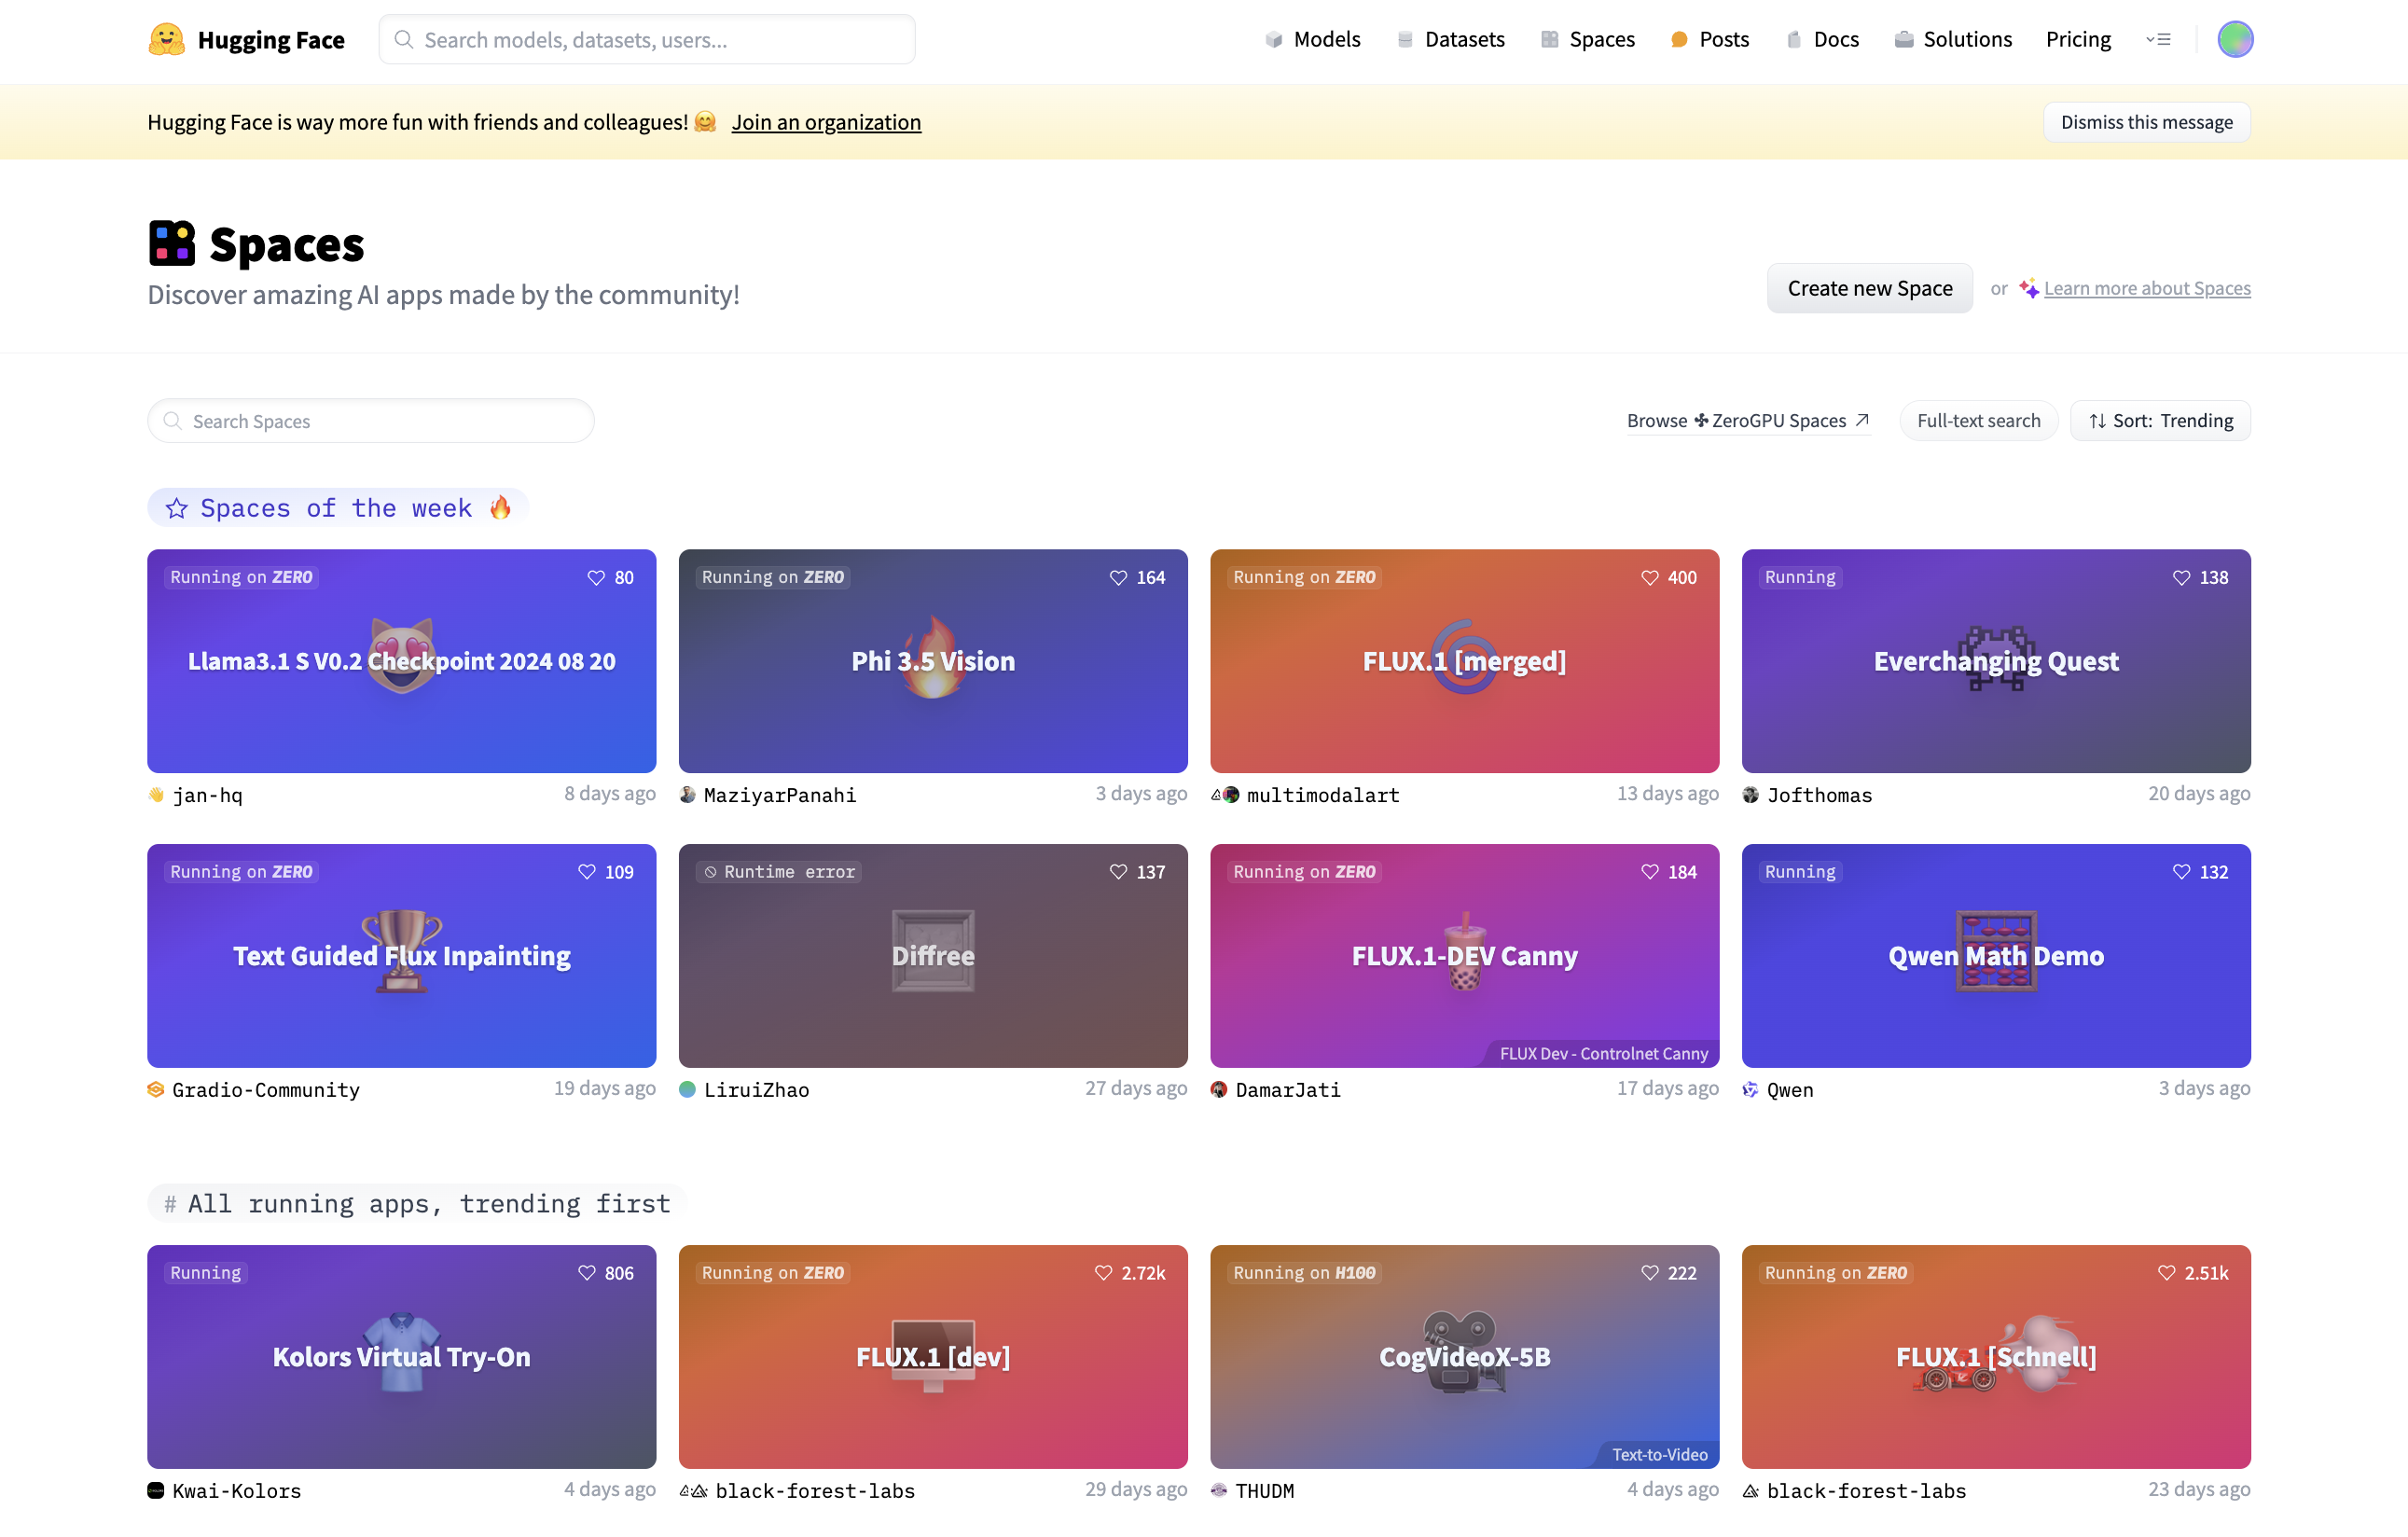
\includegraphics[width=1\textwidth,keepaspectratio]{images/hf_spaces}
        \caption{https://huggingface.co/spaces}
        \label{fig:hf_spaces}
    \end{figure}
\end{frame}


\end{document}



